\section{Method}
\label{sec:algorithm}

This section describes SEAL together with the data preparation and the descriptor construction that surround it. The method solves two problems at once, and the design gives them equal standing. The first problem is to group the entities by the shape of their target trajectory, so that a group holds entities that evolve in a similar way over time. The second problem is to describe each group by a short rule over the entity attributes, so that a reader can tell who is in a group and why. Neither problem is subordinate to the other. A grouping with tight trajectories but no simple description is of little use to a domain reader, and a rule that does not track a coherent trajectory shape explains nothing. The method therefore searches for a grouping and its description together and keeps a candidate only when both halves succeed, which is what separates it from a pipeline that clusters first and explains afterwards. Figure~\ref{fig:pipeline} gives the overall flow, and the two halves are developed in turn below before the preparation and the descriptor vocabulary that support them.

\begin{figure}[t]
\centering
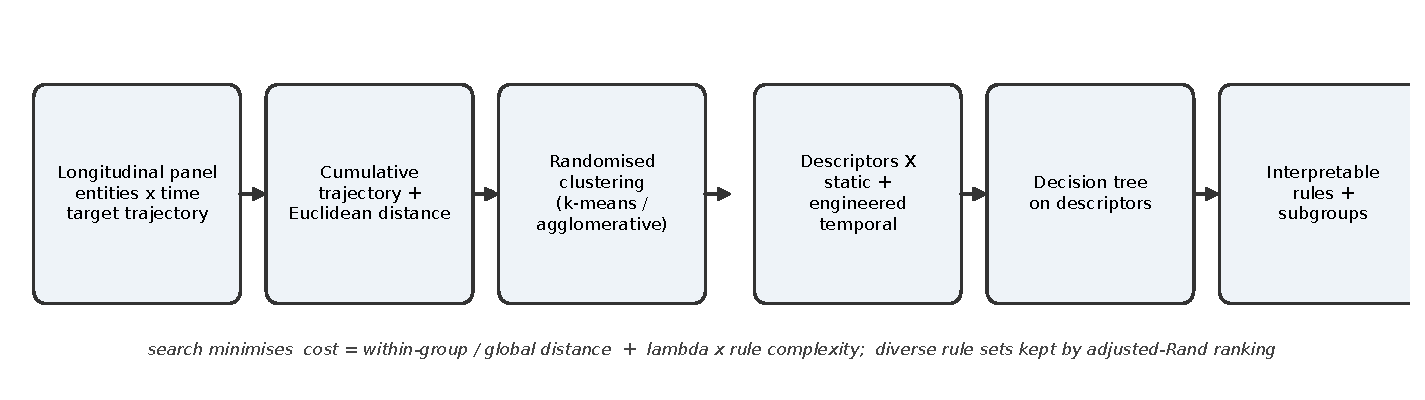
\includegraphics[width=\textwidth]{fig_pipeline.pdf}
\caption{The segmentation pipeline. A longitudinal panel is turned into a cumulative-trajectory distance, a randomised search proposes clusterings and fits a shallow decision tree to each one over the descriptor matrix, and the tree with the lowest cost is read back as an ordered rule set. The descriptor matrix carries static attributes together with engineered temporal features.}
\label{fig:pipeline}
\end{figure}

\subsection{Part one, grouping trajectories by shape}
\label{sec:distance}

Two entities are treated as similar when their target trajectories evolve in a similar way. Rather than compare the raw values point by point, the trajectory of each entity is first accumulated over time. For entity $i$ the cumulative trajectory is $\mathbf{c}_i$ with $c_{i,t} = \sum_{s \le t} y_{i,s}$. The distance between two entities is the Euclidean distance between their cumulative trajectories,
\begin{equation}
D(i,j) = \lVert \mathbf{c}_i - \mathbf{c}_j \rVert_2 .
\end{equation}
Accumulation makes the distance sensitive to the level and the persistence of a difference rather than to single-period noise, because a gap that opens up early is carried forward through every later coordinate. The average of $D$ over all pairs of entities, written $\bar{D}$, serves as a reference scale for the cost defined below.

\subsection{Proposing candidate groupings}
\label{sec:search}

The grouping is not read off a single clustering. Because the eventual goal is a grouping that a rule can also describe, the method proposes many candidate groupings and lets the second half of the problem decide among them. A single proposal is produced as follows. A number of groups $k$ is drawn from a small range. With equal probability the cumulative trajectories are grouped either by $k$-means or by agglomerative clustering, and for agglomerative clustering the linkage is itself drawn at random. The resulting group labels are a candidate grouping, one hypothesis about how the population splits by trajectory shape. Drawing many such proposals, with different group counts and different clustering rules, lets the search range over coarse and fine partitions and over compact and elongated group shapes, so that the description step is offered a wide field of groupings rather than one.

\subsection{Part two, describing each group by a rule}
\label{sec:cost}

The second half of the problem carries as much weight as the first. A candidate grouping is only worth reporting if a reader can be told, in a sentence, who belongs to each group. This half is handled by fitting a shallow decision tree on the descriptor matrix to reproduce the candidate group labels. The tree partitions the entities using axis-aligned tests on the descriptors, and the path from the root to each leaf is the conjunctive rule that names the corresponding group. Two things follow from using a tree here rather than a separate post-hoc explainer. First, every group is guaranteed a description, since the tree itself is what assigns entities to groups. Second, and more important, a grouping that no shallow tree can reproduce is effectively rejected, because the tree will fail to separate it and the resulting rules will be long and inaccurate. The requirement of a simple faithful description therefore acts as a filter on the trajectory groupings, and this is what gives the rule half equal standing with the grouping half rather than the role of a report written after the fact.

The tree is turned into text by walking every root-to-leaf path. Repeated tests on the same feature along a path are merged into the tightest interval, so a path becomes a conjunction of at most one lower bound and one upper bound per feature. The group that holds the largest number of entities is named the default group, and the remaining groups are reported as rules. Assignment for a new entity follows the rules in order and stops at the first satisfied condition, which reproduces the tree partition exactly. Figure~\ref{fig:tree} shows one such tree for the income case study, where each leaf is a subgroup and the path to it is the rule that names it.

\subsection{Coupling the two halves through one cost}
\label{sec:couple}

The two halves meet in a single cost, and the cost is what forces them to be solved together rather than in sequence. For a labelling with groups $g$, the within-group distance ratio measures how tight the trajectories are,
\begin{equation}
r = \frac{1}{\bar{D}} \cdot \operatorname{mean}\big\{ D(i,j) \;\mid\; \ell_i = \ell_j,\ i \neq j \big\},
\end{equation}
the mean pairwise distance among entities that share a label, expressed as a fraction of the population average $\bar{D}$. A ratio below one means that grouped entities are closer to one another than two entities picked at random, so a smaller ratio rewards the grouping half. The description half is scored by the complexity $c$, the total number of conditions across all rules other than the default, so a shorter rule set is preferred. The cost combines the two,
\begin{equation}
\text{cost} = r + \lambda \, c ,
\label{eq:cost}
\end{equation}
where $\lambda$ is a small weight that sets how much tightness a unit of description has to buy. A grouping that is tight but needs a long rule pays for the rule, and a grouping with a short rule but loose trajectories pays for the looseness, so the retained candidate is the one that does well on both halves at once. The candidate with the lowest cost is reported as the segmentation.

\begin{figure}[t]
\centering
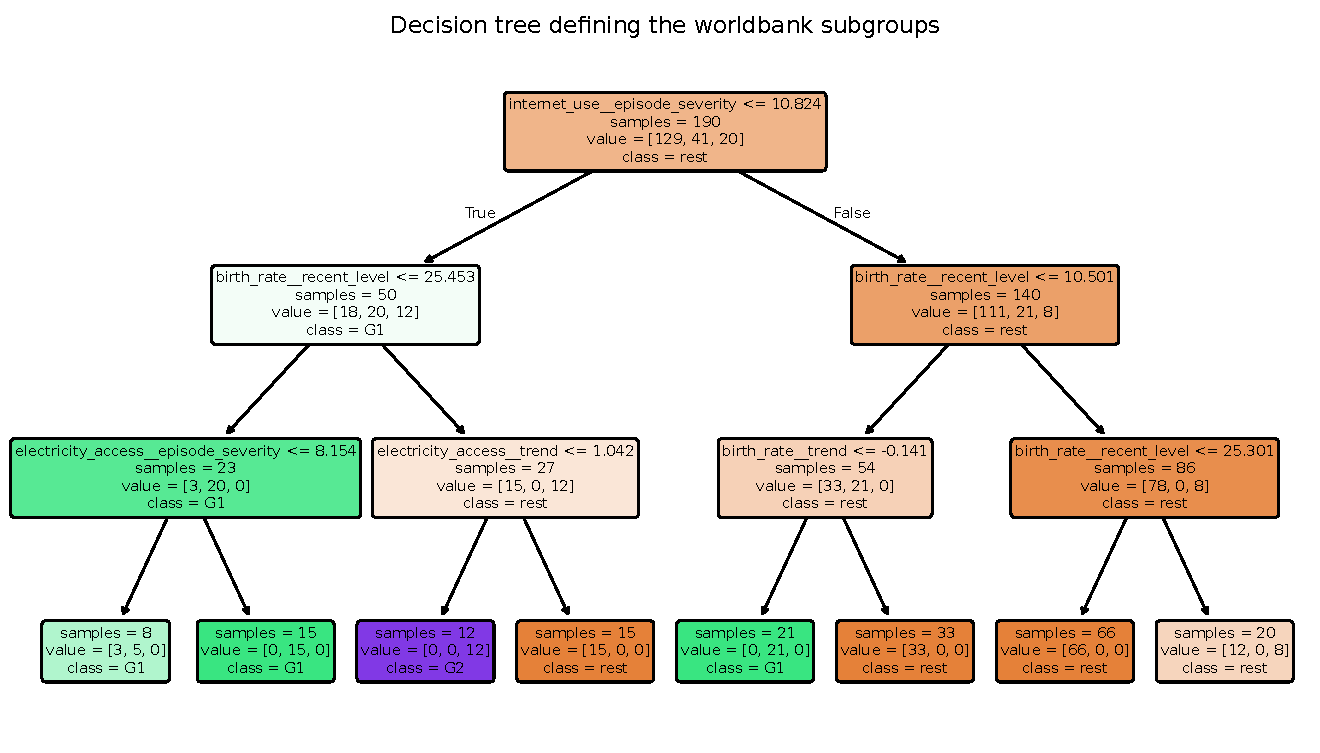
\includegraphics[width=0.9\textwidth]{fig_tree_example.pdf}
\caption{The shallow decision tree that defines the income subgroups. Each internal node tests one descriptor, each leaf is a subgroup, and the path from the root to a leaf is the conjunctive rule that names that subgroup. Reading a group off the tree and reading its rule are the same act, which is what keeps the output interpretable.}
\label{fig:tree}
\end{figure}

\subsection{Diverse rule sets}
\label{sec:diversity}

The lowest-cost candidate is rarely the only useful one. Two candidates can have almost equal cost yet describe the population in different ways, and a reader benefits from seeing genuine alternatives rather than near-duplicates. The candidates are therefore ranked by cost, and a candidate is added to the reported shortlist only when its labelling is sufficiently different from every labelling already on the shortlist. Difference is measured by the adjusted Rand index between the two labellings, and a candidate is kept when its similarity to all retained candidates stays below a fixed threshold. This yields a short list of distinct segmentations rather than many variations on one.

\begin{algorithm}[t]
\caption{Rule-based trajectory segmentation}
\label{alg:seal}
\begin{algorithmic}[1]
\Require target matrix $Y \in \mathbb{R}^{N \times T}$, descriptors $X \in \mathbb{R}^{N \times d}$, budget $M$, weight $\lambda$
\State $C \gets \text{cumulative}(Y)$; \quad $D \gets$ pairwise Euclidean distance on $C$; \quad $\bar{D} \gets \operatorname{mean}(D)$
\For{$m = 1$ to $M$}
  \State draw $k$; cluster $C$ by $k$-means or agglomerative clustering into labels $z$
  \State fit shallow decision tree $\mathcal{T}$ on $(X, z)$; let $\ell \gets \mathcal{T}(X)$
  \State $r \gets \operatorname{mean}\{ D(i,j) \mid \ell_i = \ell_j \} / \bar{D}$; \quad $c \gets$ total rule length of $\mathcal{T}$
  \State record candidate $(\ell, \mathcal{T}, \text{cost} = r + \lambda c)$
\EndFor
\State \Return lowest-cost candidate, and a diverse shortlist ranked by cost under an adjusted-Rand threshold
\end{algorithmic}
\end{algorithm}

\subsection{Target construction and data preparation}
\label{sec:preprocessing}

The target trajectory is built before any search takes place, and several choices at this stage decide what the rules can later say. Every entity is placed on a shared time grid so that the coordinates of $\mathbf{y}_i$ refer to the same calendar positions across entities. Values flagged as missing or as data-collection sentinels are removed rather than treated as zeros. Where a target is a ratio, the denominator is protected so that the ratio cannot explode. In the health case study, for example, the target is the share of income spent on health, and household-months whose income falls below a low percentile are dropped so that a near-zero denominator does not manufacture an extreme share. Right-skewed targets are passed through a logarithm of one plus the value so that ordinary variation is not drowned out by a few very large observations.

Gaps in a trajectory are handled by a completeness rule rather than by silent imputation. An entity is admitted only when it is observed across enough of the chosen window, and the few remaining internal gaps are filled by linear interpolation between observed points. Entities with large stretches of missing data are excluded rather than reconstructed, because a trajectory that is mostly invented cannot support an honest statement about shape.

\subsection{Descriptors and temporal feature engineering}
\label{sec:temporal}

Descriptors decide the vocabulary in which a subgroup can be described, so they are engineered rather than taken raw. Static attributes such as demographic counts and categorical memberships are used directly. Categorical attributes are expanded into indicator columns, one per level, so that the decision tree can split on a single category and a rule reads in plain language, for example requiring that a monitoring site be industrial. Binary attributes are kept as single indicators. Treating categorical and binary attributes as first-class descriptors matters because a rule that can only test continuous quantities cannot express membership in a named group, which is often the most actionable thing to know.

For every covariate that itself varies over time, a set of temporal features is computed so that the rules can speak about how a covariate moved rather than only about its final value. Figure~\ref{fig:temporal} illustrates the features on a single series. The linear trend summarises the direction of drift over the window. The recent level records where the covariate stands at the end of the window. The worst sustained shortfall episode captures a genuine multi-period decline rather than a single dip, and it is described by three numbers, namely how deep the shortfall ran in units of the entity's own variability, how many consecutive periods it lasted, and how long ago it ended. Where an event of interest has a known date, a datable drop feature records the largest fall inside a fixed sub-window, which lets a rule refer to a fall during a named period rather than at any time.

\begin{figure}[t]
\centering
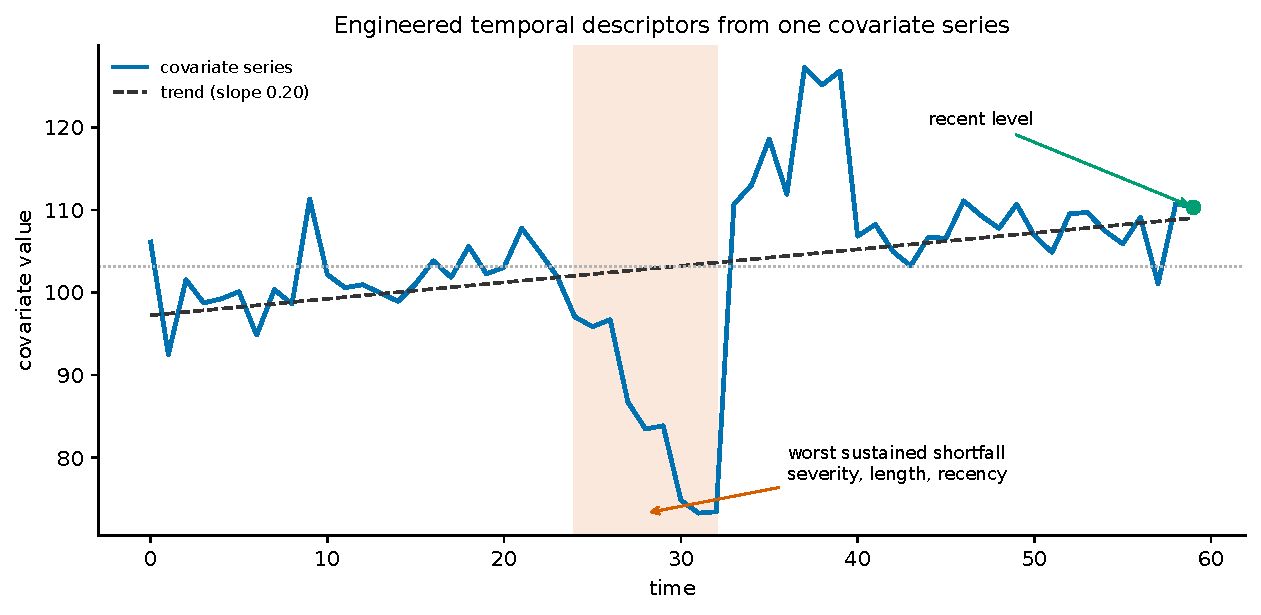
\includegraphics[width=0.8\textwidth]{fig_temporal_features.pdf}
\caption{Temporal features engineered from one covariate series. A linear trend records drift, the recent level records the ending value, and the worst sustained shortfall episode is summarised by its depth, its length, and how long ago it ended. These features let a rule describe how a covariate moved over the window rather than only its final value.}
\label{fig:temporal}
\end{figure}

\subsection{Design choices}
\label{sec:design}

We make three decisions that shape the runs reported here. First, we discard no entity by sampling. The distance matrix grows with the square of the number of entities, yet the panels studied here are small enough that we keep every entity, which removes a source of instability in which the discovered rules would depend on which entities happened to be drawn. The health case study has a larger entity count, and there too we use the full admitted cohort rather than a subsample.

Second, we hold the descriptors to a strict non-circularity rule. No descriptor may be the target or a quantity mechanically derived from it. In the health case study the target is health spending divided by income, so we forbid health-spending columns as descriptors, and we forbid the income level as well because it is the denominator of the target. We keep income dynamics such as trends and shortfalls, since a statement about how income moved is not a restatement of the target. Without this rule a search would rediscover the definition of the target and present it as an insight.

Third, we compute temporal features over the same window as the target rather than over each entity's full history. If the target describes a fixed period, then a descriptor that counts income shortfalls should count them inside that period as well, otherwise a rule can appear to explain the window using events from outside it.
